% !TEX root = ../main.tex
% \begin{center}
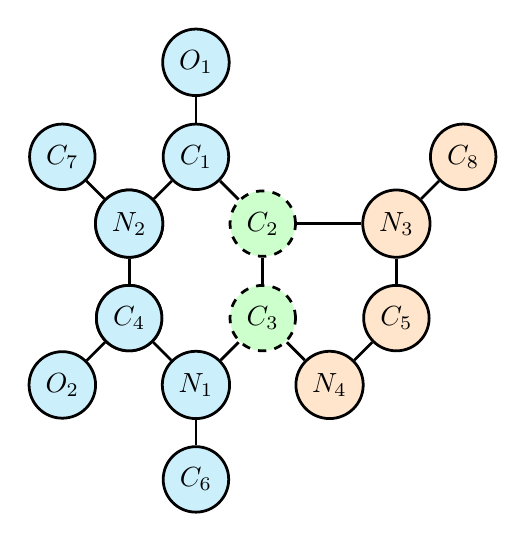
\begin{tikzpicture}[node distance={12mm}, line width=1pt, main/.style = {draw, circle}] 
\node[main,fill=cyan!20] (1) []{$C_1$}; 
\node[main, fill=green!20, dashed] (2) [below right of=1]{$C_2$}; 
\node[main, fill=green!20, dashed] (3) [below of=2]{$C_3$}; 
\node[main,fill=cyan!20] (4) [below left of=3]{$N_1$}; 
\node[main,fill=cyan!20] (5) [above left of=4]{$C_4$}; 
\node[main,fill=cyan!20] (6) [above of=5]{$N_2$};
\node[main,fill=orange!20] (9) [below right of=3]{$N_4$}; 
\node[main,fill=orange!20] (8) [above right of=9]{$C_5$}; 
\node[main, fill=orange!20] (7) [above of=8]{$N_3$};
\node[main,fill=cyan!20] (10) [above of=1]{$O_1$}; 
\node[main,fill=cyan!20] (11) [above left of=4]{$C_4$}; 
\node[main,fill=cyan!20] (12) [above of=5]{$N_2$}; 

\node[main,fill=cyan!20] (13) [below of=4]{$C_6$};  

\node[main,fill=cyan!20] (17) [below left of=5]{$O_2$};

\node[main,fill=cyan!20] (18) [above left of=6]{$C_7$}; 

\node[main,fill=orange!20] (22) [above right of=7]{$C_8$}; 



\draw [] (1) -- (2); 
\draw [] (2) -- (3); 
\draw [] (3) -- (4); 
\draw [] (4) -- (5); 
\draw [] (5) -- (6); 
\draw [] (6) -- (1); 
\draw [] (2) -- (7); 
\draw [] (7) -- (8); 
\draw [] (8) -- (9); 
\draw [] (9) -- (3); 
\draw [] (1) -- (10); 

\draw [] (4) -- (13); 

\draw [] (5) -- (17); 

\draw [] (6) -- (18); 

\draw [] (7) -- (22); 
\end{tikzpicture}
% \end{center}
